

Various integrity verification methods have been developed to reduce communication and computational overhead. The overhead imposed by Message Authentication Codes (MACs) is a significant issue in bandwidth-limited networks such as CAN~\cite{compoundMAC} and in high data rate applications within 5G networks~\cite{etsi_ts_133501_v17_5_0}. Truncated MACs have been proposed as a practical solution to mitigate this overhead. However, truncation comes at the expense of security strength, making the system more vulnerable to collision attacks~\cite{ProMAC1}.

Other overhead-reducing schemes, such as aggregate and compound MACs, minimize computational and communication overhead by verifying multiple messages with a single tag. While this approach eliminates the need to compute and transmit a MAC for every individual message, it introduces a critical weakness: the loss or corruption of any single packet within the group prevents the integrity verification of the entire set. This weakness arises because all messages contribute to the generation of the common MAC, making them mutually dependent. Consequently, the integrity check fails if even one message is missing, leaving the common MAC unusable.

To address this weakness, it is important to recognize that aggregate and compound MAC schemes were originally designed for error-free communication links, which makes them particularly susceptible to packet losses. Such losses may arise naturally in lossy channels or be deliberately introduced through jamming attacks, indicating the presence of an adversary~\cite{jamming_Servey, XOR_MAC, proMac2, DoS_AggregateMAC}. Detecting and preventing jamming is especially challenging in wireless environments. Random jamming, for example, mimics the behavior of a naturally lossy channel, making reliable detection extremely difficult~\cite{jamming_Servey}. Therefore, MAC overhead-reducing schemes must explicitly consider the impact of various jamming strategies, including random and periodic jamming, to ensure resilience under adversarial conditions.
% For example, if aggregate or compound MACs are implemented, an attacker can execute denial-of-service (DoS) attacks by jamming every $'n'$ packets. This is a much lower rate compared to that of traditional MACs~\cite{DoS_AggregateMAC, XOR_MAC}. Since the modification of a single packet in aggregated MAC schemes can prevent the verification of multiple messages due to their interdependencies, the attacker can significantly disrupt communication with minimal effort.
In this context, assessing the message-to-tag dependencies becomes essential to maintain the integrity and availability of the system in the presence of a jammer. Understanding these dependencies is vital for designing robust integrity verification schemes that can withstand packet losses and malicious attacks.


\subsection{Problem Background}
The earliest integrity-check overhead reduction approach can be traced to \cite{XOR_MAC_original}, which introduced an XOR-based aggregation technique that combines multiple digital signatures into a single compact signature. This method not only reduces the total size of transmitted signatures but also provides provable security guarantees\cite{boneh2003aggregate, XOR_MAC_original, XOR_MAC}. Building on this idea, \cite{aggregateMAC}~has applied the aggregation technique to MAC schemes, combining multiple tags into a single tag to reduce communication overhead. An alternative direction, explored in~\cite{sequential_aggregate, sequential_aggregate2, application_sequential_aggregation}, proposed sequential aggregation, where each new signature is computed over the current message concatenated with the preceding signature, effectively chaining multiple signatures into one. 
\begin{figure}[h]
    \centering
    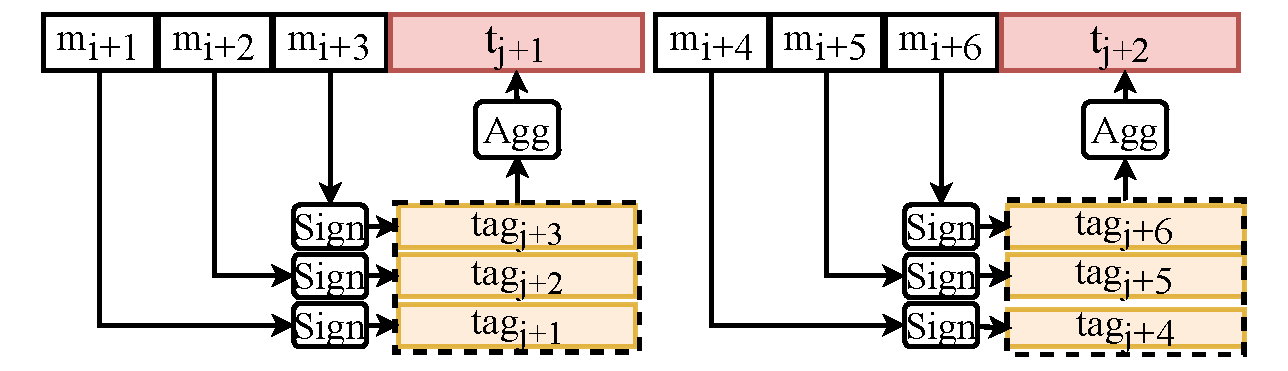
\includegraphics[width= \columnwidth]{img/MAC/AggMAC.pdf}
    \caption{Aggregate MAC~\cite{aggregateMAC}}
    \label{fig:AggMAC}
\end{figure}

Figure~\ref{fig:AggMAC} illustrates the MAC aggregation technique proposed in~\cite{aggregateMAC}. Alternative approach, as shown in Figure~\ref{fig:AggMAC}, involves aggregating messages to generate a single tag, transmitting the resulting tag for all aggregated messages~\cite{compoundMAC, stateful, compundMAC_original, miniMAC}. 
\begin{figure}[h]
     \centering
     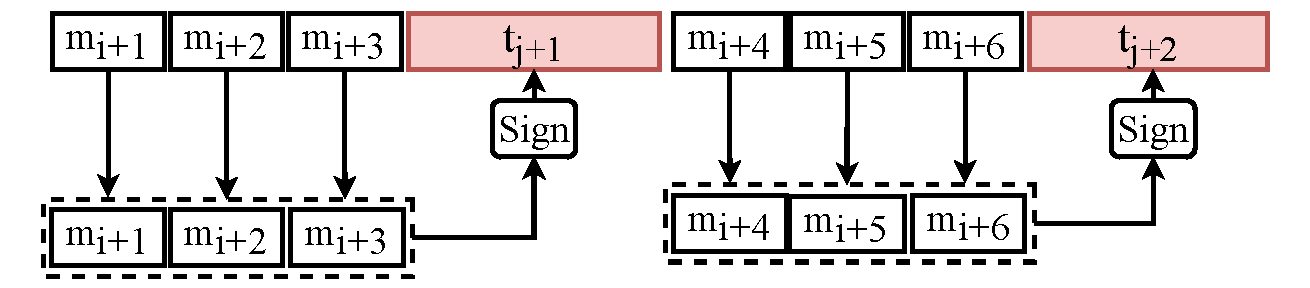
\includegraphics[width = \columnwidth]{img/MAC/CompMAC.pdf}
     \caption{Aggregate Messages~\cite{compundMAC_original}}
     \label{fig:compoundMAC}
\end{figure}
The 'Sign' operation indicates the MAC generation process, and 'Agg' depicts the aggregation step. While these two schemes are different in nature, from the message and MAC interdependency point of view, they behave the same. Thus, from now on, the aggregate MAC and aggregate message terminology might be used interchangeably.
 

 
% Our analysis focuses on the dependencies created during the aggregation step. Both aggregation approaches introduce similar vulnerabilities to packet losses. These dependencies can be exploited in jamming scenarios, leading to a significant risk of denial-of-service and reduced quality of service.

% \subsection{Related work}

In~\cite{ProMAC1}, the Progressive MACs framework is introduced, which provides a novel approach to generalize all the previous MAC aggregation schemes. Progressive MACs framework utilizes an internal state mechanism that is updated with every new message and a tag generation mechanism that inputs from the internal state. Figure~\ref{fig:proMAC} illustrates one possible realization of a progressive MAC framework, called Whips, with an internal state of size three.
\begin{figure}[h]
    \centering
    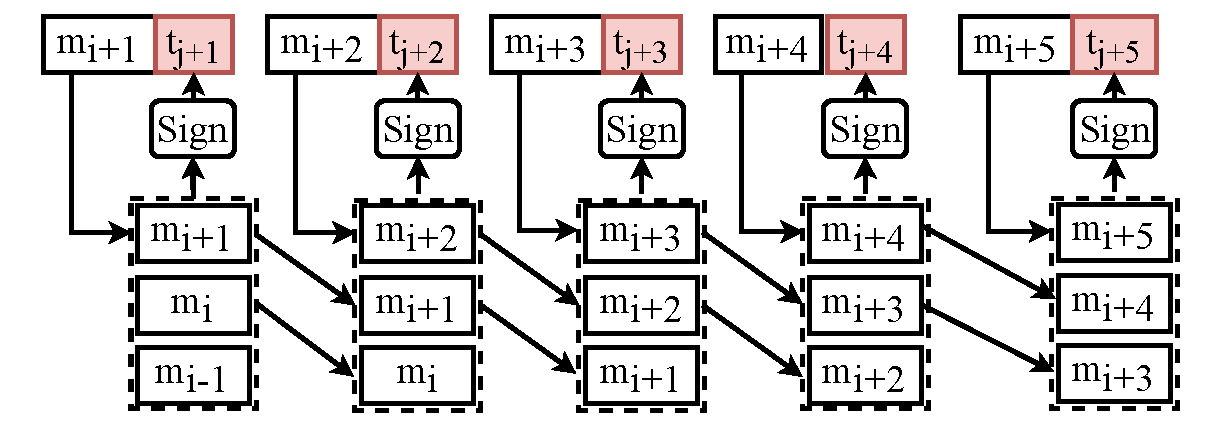
\includegraphics[width = \columnwidth]{img/MAC/ProMAC.pdf}
    \caption{ProMACs~\cite{ProMAC1, cuMAC} cross-assigns message to tag. This Figure is reproduced from~\cite{proMac2}.}
    \label{fig:proMAC}
\end{figure}
As shown in Figure~\ref{fig:proMAC}, the message $m_{i+1}$ is involved in the generation of tags $t_{j+1}$, $t_{j+2}$, and $t_{j+3}$. This way, the message $m_{i+1}$ will be verified by the three tags, which means to successfully modify $m_{i+1}$, an attacker would need to guess all three tags correctly, equivalent in security to using a tag three times as large. For instance, if a message requires the security level of a 256-bit tag, a Progressive MAC with a state of size three could achieve this with 86-bit tags, as each message is verified three times. This state mechanism allows Whips to gradually verify the integrity of packets as more tags are received, effectively increasing the security level over time without requiring full-length tags for each packet~\cite{ProMAC1}.

Therefore, Progressive MAC-based schemes~\cite{ProMAC1, proMac2, cuMAC, miniMAC} are not confined to fixed-length tag configurations. Depending on security requirements and bandwidth constraints, they can employ truncated tags that, through cumulative verification across multiple packets, offer security guarantees comparable to traditional MACs~\cite{ProMAC1}. By tuning parameters such as tag length, state-update rules, and internal state size, the Progressive MAC framework can adjust to application constraints~\cite{ProMAC1}. However, despite this versatility, the ProMAC framework lacks a systematic method for determining optimal parameter choices for different application constraints. Without a systematic approach, designing a good-performing system becomes extremely difficult. This is even more critical in adversarial environments, where periodic or random packet loss can severely attack the integrity check scheme.
 
To address this limitation, we propose OptiMAC, a graph-based mapping approach that enables a systematic design and analysis of the ProMAC framework. This graph-based method systematically analyzes and adjusts dependencies between messages and tags, resulting in an optimized structure that maximizes the number of verifiable packets under conditions of high packet loss, achieving optimal security tailored to specific channel conditions.



\subsection{Limitations in Adversarial Environments}
% The proposed methods are promising solutions for MAC overhead reduction but are not designed for lossy channels.
% In~\cite{when_And_How_Aggregate_In_Lossy_Channel}, they have studied the effect of the packet loss on the mentioned schemes where they concluded that channel condition has a remarkable influence on performance. For instance, in the Aggregate MAC, as can be seen from Figure~\ref{fig:AggMAC}, if any of the messages in the group of $\{m_{i+1}, m_{i+2}, m_{i+3}\}$ is lost or modified, the other messages will not be verified and may be discarded.
The limitations of MAC or message aggregation schemes in adversarial scenarios have been previously pointed out. Kolesnikov et al.~\cite{DoS_AggregateMAC} demonstrated that MAC overhead-reducing schemes can increase the system's vulnerability to DoS attacks. To address this, Kolesnikov et al. proposed a "shifted bitwise XOR" approach to mitigate the impact of packet loss on the verification of other messages~\cite{DoS_AggregateMAC}.

Wagner et al.~\cite{proMac2}, introduce SP-MAC, a resilience-oriented authentication scheme extending the Progressive MAC (ProMAC) framework with a combinatorial construction based on Golomb rulers and generalized $g$-Sidon sets~\cite{proMac2}. This dependency structure is designed to limit the effect of a message loss on the other messages, making it more resilient in adversarial scenarios. Despite the SP-MAC claim of having the \emph{optimal} dependency distribution, it lacks quantifiable objectives. The provable guarantees are controllable latency and controllable effect of message-loss on other messages. Though this doesn't by it self guarentee optimal latency or optimal goodput of the overall system. Moreover, Similar to many other schemes, the number of tags that are required to be genereted equals to the number of messages, whereas aggregate MAC and Our proposed OptiMAC allow flexibility on the number of tag used per message, reducing computational overhead. 

It is evident from~\cite{proMac2, DoS_AggregateMAC, when_And_How_Aggregate_In_Lossy_Channel} that grouping messages or aggregating tags to reduce overhead introduces verification dependencies between messages. These dependencies can add latency and make the system vulnerable to jamming. While some prior work~\cite{DoS_AggregateMAC, proMac2} has recognized this problem and proposed heuristic solutions, our study presents an optimization approach to find the optimal parameters in adversarial environments.

In summary, progressive MAC introduces a framework that generalizes all MAC aggregation schemes through an evolving internal state and an arbitrary update and tag generation function. However, the lack of guidance to find the optimum settings for this framework, especially in challenging under-attack environments, leaves a gap that we are addressing in this paper. Our proposed OptiMAC framework maps the state and the update functions of the ProMAC framework to a graph, providing a systematic approach to analyze and optimize any MAC aggregation schemes. Addressing this issue is critical for improving the efficiency and security of communication systems, particularly in adversarial wireless environments. 


%Based on this mapping we develop an optimization model enables to also application of different MAC schemes under varying conditions, offering robust guidance for designing more resilient wireless communication systems.


% A critical research gap exists in finding the optimal dependency distribution between tags and messages to maximize verified throughput and minimize latency in lossy channels. This paper addresses this issue by systematically studying the dependency problem, aiming to optimize the verification process for different channel conditions.
% The current methods, while effective in reducing overhead, often introduce dependencies that can lead to increased latency and vulnerability to attacks, especially in environments with high packet loss rate. 










